% =====================================================================
%  CIE 555 - Project presentation (Beamer)
%  Compile:  pdflatex slides.tex   (run twice)
% =====================================================================
\documentclass[aspectratio=169,11pt]{beamer}

\usetheme{Madrid}
\usecolortheme{whale}
\setbeamertemplate{navigation symbols}{}
\setbeamertemplate{caption}{\raggedright\insertcaption\par}

\usepackage[utf8]{inputenc}
\usepackage[T1]{fontenc}
\usepackage{lmodern}
\usefonttheme{professionalfonts}  % use standard math fonts (avoids MiKTeX sans-math font issue)
\usepackage{graphicx}
\usepackage{booktabs}

\title[GEC on C4\_200M]{Grammatical Error Correction on C4\_200M}
\subtitle{Bag-of-Words \textrightarrow{} LSTM \textrightarrow{} Attention \textrightarrow{} Transformer}
\author[Ahmed \& Hanafy]{Abdullah Ahmed (202200206) \and Ibrahim Hanafy (202200518)}
\institute[CIE 555]{CIE 555 --- Neural Networks and Deep Learning\\
\footnotesize Instructor: Dr.\ Ibrahim Swelam \quad TAs: Aya Abdelaziz, Mahmoud Farahat}
\date{May 2026}

\begin{document}

% ---------------------------------------------------------------- 1
\begin{frame}\titlepage\end{frame}

% ---------------------------------------------------------------- 2
\begin{frame}{The Problem: Grammatical Error Correction}
Rewrite an ungrammatical sentence into its corrected form.
\vspace{1em}
\begin{block}{Example}
\textbf{Input (corrupted):} \emph{``She go to school yesterday and learning many thing.''}\\[4pt]
\textbf{Output (corrected):} \emph{``She went to school yesterday and learned many things.''}
\end{block}
\vspace{0.5em}
\begin{itemize}
  \item Errors: verb tense, agreement, articles, plurals, punctuation, spelling.
  \item The output is a \textbf{whole new sentence} --- a sequence-to-sequence task.
\end{itemize}
\end{frame}

% ---------------------------------------------------------------- 3
\begin{frame}{The Data: C4\_200M Subset}
\textbf{C4\_200M} --- clean web text automatically corrupted into
\texttt{(corrupted, clean)} pairs.
\vspace{0.8em}
\begin{columns}
\begin{column}{0.5\textwidth}
\begin{tabular}{lr}
\toprule
Split & Pairs \\
\midrule
Train      & 850{,}000 \\
Validation & 50{,}000 \\
Test       & 100{,}000 \\
\midrule
Total      & 1{,}000{,}000 \\
\bottomrule
\end{tabular}
\end{column}
\begin{column}{0.5\textwidth}
\begin{itemize}
  \item 16k Byte-Level BPE tokenizer.
  \item Max length 64 tokens.
  \item Same splits + tokenizer for every model (no leakage).
\end{itemize}
\end{column}
\end{columns}
\end{frame}

% ---------------------------------------------------------------- 4
\begin{frame}{Four Models of Increasing Power}
\begin{tabular}{cll}
\toprule
\# & Model & What it adds \\
\midrule
1 & Bag-of-Words (TF--IDF) & Baseline --- only \emph{detects} errors \\
2 & LSTM encoder--decoder  & First corrector; fixed-size bottleneck \\
3 & LSTM + Bahdanau attn   & Decoder re-queries the full source \\
4 & Transformer            & Self-attention; no recurrence \\
\bottomrule
\end{tabular}
\vspace{1em}
\begin{center}
\small Model 1 \emph{detects}. Models 2--4 \emph{correct}.
\end{center}
\end{frame}

% ---------------------------------------------------------------- 5
\begin{frame}{Model 1 --- Bag-of-Words Baseline}
TF--IDF (unigrams+bigrams, 50k vocab) + Logistic Regression / Linear SVM.
Each pair \textrightarrow{} two samples: corrupted = 0, clean = 1.
\vspace{0.5em}
\begin{block}{Result: $\sim$62\,\% accuracy --- barely above 50\,\% chance}
\small Why so weak? It is \emph{structural}, not bad tuning:
\begin{itemize}\small
  \item \textbf{Detector, not corrector} --- outputs one label, can never
        produce corrected text.
  \item \textbf{Bag-of-words discards order} --- but grammar \emph{is} order
        (``she goes'' vs ``go she'').
  \item \textbf{Error signal swamped} --- a 1-word error is invisible next to
        content-word TF--IDF weights.
  \item \textbf{No generalisation} --- only memorises lexical statistics.
\end{itemize}
\end{block}
\centering \small Proves GEC needs sequence modelling + generation.
\end{frame}

% ---------------------------------------------------------------- 6
\begin{frame}{Model 2 --- LSTM Encoder--Decoder}
\begin{columns}
\begin{column}{0.55\textwidth}
\begin{itemize}
  \item BiLSTM encoder compresses input into \textbf{one} 512-dim state.
  \item LSTM decoder generates the correction token by token.
  \item Teacher forcing $1.0 \to 0.5$; 19.55\,M params; 3 epochs.
\end{itemize}
\end{column}
\begin{column}{0.45\textwidth}
\begin{block}{The bottleneck}
After the first step the decoder never ``sees'' the source again ---
everything is squeezed into 512 numbers.
\end{block}
\end{column}
\end{columns}
\vspace{0.6em}
\centering Test GLEU \textbf{0.213} (greedy) --- weakest corrector.
\end{frame}

% ---------------------------------------------------------------- 7
\begin{frame}{Model 3 --- LSTM + Bahdanau Attention}
Keep \emph{all} encoder states; the decoder attends to them every step.
\vspace{0.6em}
\[
\text{score}(s_t,h_i)=v^{\top}\tanh(W_s s_t + W_h h_i),\quad
\alpha=\mathrm{softmax}(\text{score}),\quad
c_t=\textstyle\sum_i \alpha_{t,i} h_i
\]
\begin{itemize}
  \item Removes the bottleneck; alignment weights are interpretable.
  \item Padding masked with $-\infty$ before softmax.
  \item 29.06\,M params.
\end{itemize}
\begin{block}{Result --- the decisive jump}
GLEU \textbf{0.213 \textrightarrow{} 0.599} ($+0.386$). Attention matters most.
\end{block}
\end{frame}

% ---------------------------------------------------------------- 8
\begin{frame}{Model 4 --- Transformer}
\begin{columns}
\begin{column}{0.55\textwidth}
\begin{itemize}
  \item No recurrence --- self-attention only.
  \item $d_{\text{model}}{=}256$, 8 heads, 3+3 layers, FFN 512.
  \item Sinusoidal positional encoding; causal mask in decoder.
  \item Label smoothing 0.1; warmup LR; weight tying.
\end{itemize}
\end{column}
\begin{column}{0.45\textwidth}
\begin{block}{Smallest \& strongest}
Only \textbf{8.05\,M} params (3.6$\times$ fewer than Model 3).\\
Best validation GLEU \textbf{0.613}.
\end{block}
\end{column}
\end{columns}
\vspace{0.4em}
\centering \small Self-attention: every token directly attends to every other ---
$O(1)$ path length, fully parallel.
\end{frame}

% ---------------------------------------------------------------- 9
\begin{frame}{Comparative Results --- Test Set}
\centering
\begin{tabular}{l c c c c}
\toprule
Model & Decoding & Params & EM & GLEU \\
\midrule
LSTM (no attention) & greedy & 19.55\,M & $\approx$0.008 & 0.213 \\
LSTM (no attention) & beam-4 & 19.55\,M & --             & 0.256 \\
LSTM + Bahdanau     & greedy & 29.06\,M & 0.024          & 0.599 \\
LSTM + Bahdanau     & beam-4 & 29.06\,M & 0.026          & \textbf{0.618} \\
Transformer         & greedy & 8.05\,M  & 0.022          & \textbf{0.618} \\
Transformer         & beam-4 & 8.05\,M  & 0.020          & \textbf{0.618} \\
\bottomrule
\end{tabular}
\vspace{0.8em}
\begin{itemize}\small
  \item Beam search helps the LSTM, not the (well-calibrated) Transformer.
  \item Transformer ties Model 3 on GLEU with 3.6$\times$ fewer parameters.
\end{itemize}
\end{frame}

% ---------------------------------------------------------------- 10
\begin{frame}{Attention Is Interpretable}
\begin{columns}
\begin{column}{0.5\textwidth}
\centering
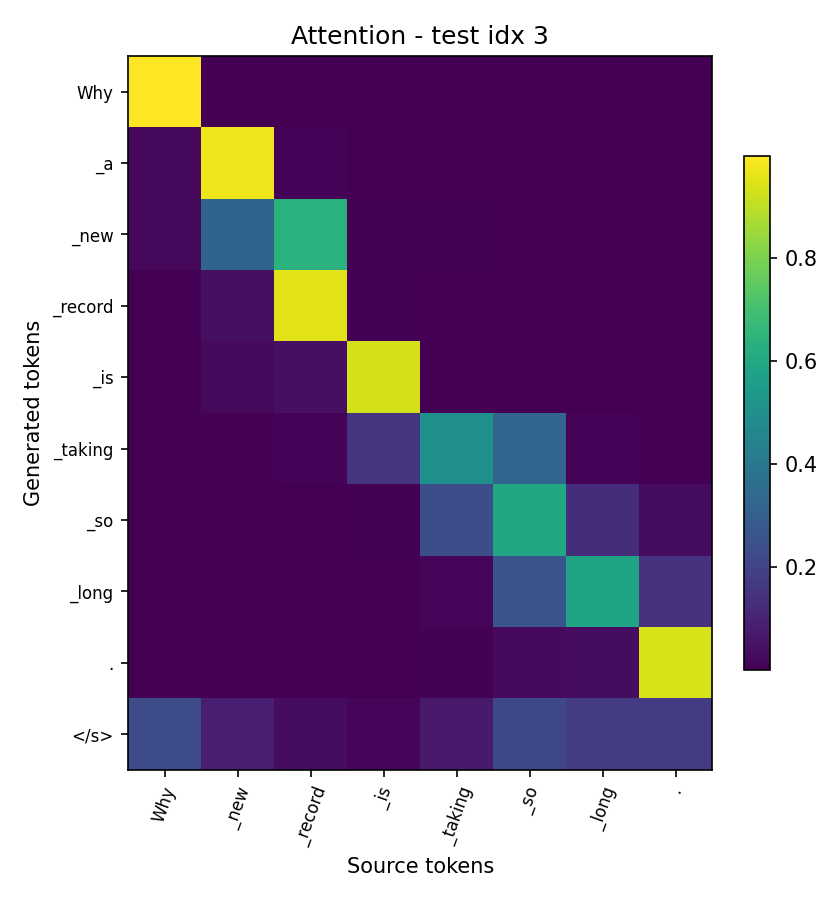
\includegraphics[width=\textwidth]{../report/figures/attn_3.png}\\
\small Bahdanau decoder alignment
\end{column}
\begin{column}{0.5\textwidth}
\centering
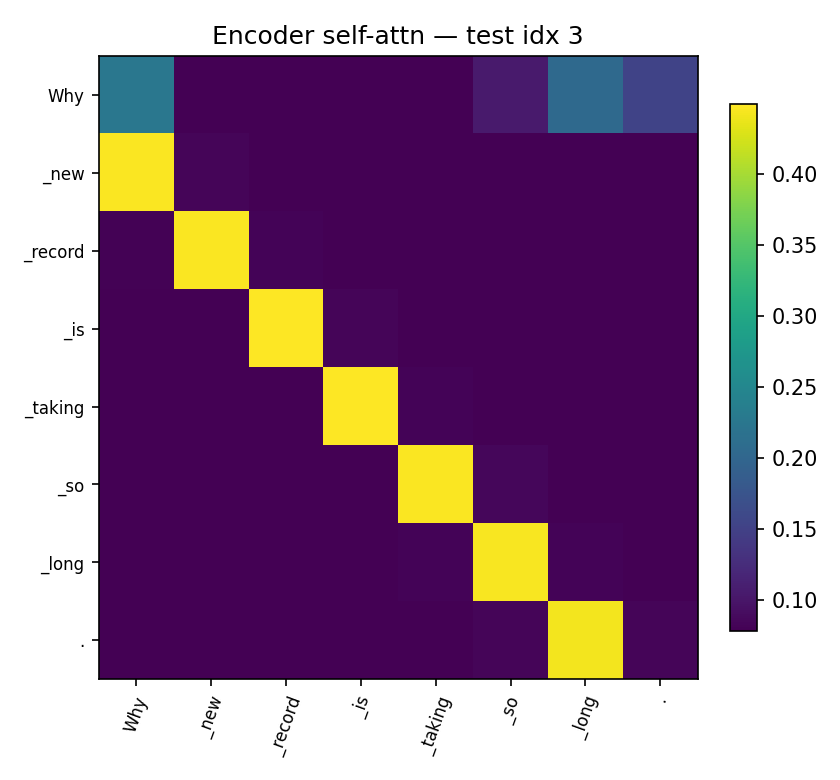
\includegraphics[width=\textwidth]{../evaluation/phase5_transformer/enc_self_attn_3.png}\\
\small Transformer encoder self-attention
\end{column}
\end{columns}
\vspace{0.5em}
\centering \small Bright cells = which source token the model focuses on.
\end{frame}

% ---------------------------------------------------------------- 11
\begin{frame}{Behaviour by Sentence Length}
\centering
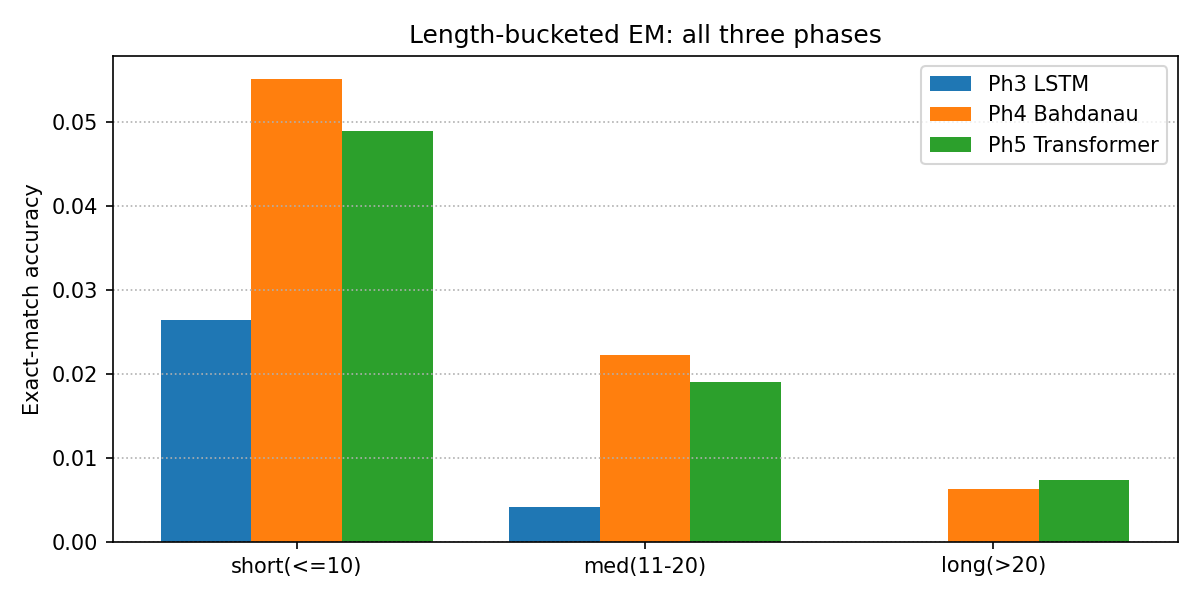
\includegraphics[width=0.62\textwidth]{../evaluation/phase5_transformer/three_way_compare.png}
\vspace{0.2em}
\begin{itemize}\small
  \item Bottleneck LSTM (blue) collapses to $\approx$0 on medium/long sentences.
  \item Bahdanau \& Transformer stay non-zero everywhere --- attention is what
        prevents the collapse.
  \item \textbf{Crossover:} Transformer (green) overtakes Bahdanau (orange) on
        the \emph{long} bucket --- its $O(1)$ path helps most there.
\end{itemize}
\end{frame}

% ---------------------------------------------------------------- worked ex
\begin{frame}[fragile]{Worked Example --- The Three Correctors}
\textbf{Short sentence} (insert a missing article):
{\footnotesize
\begin{verbatim}
SRC : Why new record is taking so long.
REF : Why the new record is taking so long.
P3  : Why new record is taking so long.   LSTM  - no edit (copies)
P4  : Why a new record is taking so long. Bahd. - inserts article "a"
P5  : Why new record is taking so long?   Trans.- "." -> "?"
\end{verbatim}}
\textbf{Long, noisy sentence:}
{\footnotesize
\begin{verbatim}
P3 : "...cpue to buy and/indukine stead..."  hallucinated nonsense
P4 : copies source, corrupts the URL
P5 : copies source, fixes "got" -> "get"     the one real fix
\end{verbatim}}
\centering \small LSTM collapses on long input; P4 \& P5 differ by 1--2 tokens.
\end{frame}

% ---------------------------------------------------------------- P4 vs P5
\begin{frame}{Why Bahdanau LSTM $\approx$ Transformer}
Test GLEU is tied at \textbf{0.618}. The Transformer \emph{matches}, not beats:
\begin{enumerate}
  \item \textbf{Decisive feature is shared} --- both have full source access via
        attention (the +0.386 jump). LSTM-vs-self-attention is second-order.
  \item \textbf{Both hit the data ceiling} --- same budget, same noisy C4\_200M
        references \textrightarrow{} both converge to GLEU $\approx$0.62.
  \item \textbf{Sentences are mostly short} --- the Transformer's $O(1)$ path
        only helps on long-range deps (see the crossover).
  \item \textbf{On hard inputs both just copy} --- outputs differ by 1--2 tokens.
\end{enumerate}
\begin{block}{The real win is efficiency}
Same quality with \textbf{8.05\,M} params vs 29.06\,M ($3.6\times$ fewer) +
faster parallel training --- it would pull ahead with more data / cleaner refs.
\end{block}
\end{frame}

% ---------------------------------------------------------------- 12
\begin{frame}{Grammar-Rule Analysis of Outputs}
\textbf{Learned well} (local syntax):
\begin{itemize}\small
  \item Subject--verb agreement: \emph{``What are this job''} \textrightarrow{} \emph{``What is this job''}
  \item Articles: \emph{``Why new record''} \textrightarrow{} \emph{``Why the new record''}
  \item Verb tense, punctuation, spacing.
\end{itemize}
\vspace{0.4em}
\textbf{Still hard:}
\begin{itemize}\small
  \item Long-range / semantic edits; rare-word spelling (hallucination).
  \item Dominant failure = \emph{under-correction}: copying the source unchanged
        (the safe, high-probability action).
\end{itemize}
\end{frame}

% ---------------------------------------------------------------- 13
\begin{frame}{The Final Challenge --- Dataset Quality}
Why does \textbf{every} model score only $\sim$2\,\% exact match?
\vspace{0.6em}
\begin{block}{Reference quality is the ceiling --- not model capacity}
\small
\textbf{1. References are paraphrases:} \emph{``informed''}\,\textrightarrow{}\,\emph{``suggest''},
\emph{``startups''}\,\textrightarrow{}\,\emph{``start-ups''} --- not grammar errors.\\[3pt]
\textbf{2. References can be noisy:} target \emph{``no brain worky''} --- ``worky''
is not a word.\\[3pt]
\textbf{3. Many valid corrections exist;} EM credits exactly one.
\end{block}
\centering \small
\textrightarrow{} Report GLEU / $F_{0.5}$, not EM. Cleaner data would help more
than a bigger model.
\end{frame}

% ---------------------------------------------------------------- 14
\begin{frame}{Conclusion}
\begin{itemize}
  \item \textbf{BoW} detects grammaticality at $\sim$62\,\% --- cannot correct.
  \item \textbf{LSTM} corrects but is limited by the bottleneck (GLEU 0.213).
  \item \textbf{Bahdanau attention} is the decisive jump (GLEU 0.599).
  \item \textbf{Transformer} ties on GLEU (0.618) with 3.6$\times$ fewer params
        and best validation GLEU (0.613).
\end{itemize}
\vspace{0.6em}
\begin{block}{Key insight}
The binding constraint is \textbf{dataset quality}, not architecture ---
synthetic C4\_200M references are often paraphrases or noise.
\end{block}
\end{frame}

% ---------------------------------------------------------------- 15
\begin{frame}
\centering \Large Thank you \\[6pt]
\normalsize Questions?
\end{frame}

\end{document}
